\chapter{Theory}

    Humans have been concerned with the fundamental nature and constituents of matter since as early as sixth century BC, when philosophers such as Democritus and Leucippus {\color{red} cite} first proposed indivisible building blocks of nature known as ``atoms.'' It wasn't until Dalton in the nineteenth century when scientific modeling of the particle nature began to take shape {\color{red} cite}. Fundamental advances on the nature of atoms were made over the next centuries by Mendeleev, Thomson, Rutherford, amongst others. Over the 1950s and 1960s, with the advent of scattering experiments, many particles were discovered forming what was known as the ``particle zoo.'' In order to classify these particles, Murray Gell-Mann proposed the quark model
    

    \section{The Standard Model}

        The \gls{SM} of particle physics is a theory which describes the particles and interactions in the universe. It was developed throughout the later half of the 20th century
        
        % todo figure out where to put this        
        The standard model Lagrangian is given by:

        \begin{equation}
            \begin{aligned}
                \mathcal{L} &= - \frac{1}{4} F_{\mu \nu} F^{\mu \nu} \\
                &=+ i \bar{\psi} \cancel{D} \psi + h.c. \\
                &=+ \bar{\psi}_i y_{ij} \psi_j \phi + h.c. \\
                &=+ |D_\mu \phi|^2 - V(\phi)
            \end{aligned}
        \end{equation}

        Where the first term describes the strong for the gluon and the strong nuclear force, the second describes the weak nuclear force along with the W and Z bosons... 

        \subsection{Fermions}
        Fermions are pin-$\frac{1}{2}$ particles which obey the Pauli Exclusion principle, and thus take up space and make up matter. Within the \gls{SM}, there are two types of fermions, quarks and leptons. Each of these can be broken down into three generations of particles.

        Quarks have several properties:
        \begin{itemize}
            \item Flavor - There are 6 flavors of quarks: up (u), down (d), strange (s), charm (c), bottom (b), and top (t) (from lightest to heaviest). Each particle also has a corresponding anti-particle: anti-up ($\bar{u}$), anti-down ($\bar{d}$), etc.
            \item Electric Charge - Quarks either have charge of $\frac{2}{3}$ (up, charm, top) or $-\frac{1}{3}$ (down, strange, bottom), while anti-quarks have the opposite charge. 
            \item Color Charge - Each quark has a degree of freedom known as color charge, which can be `red', `blue', or `green', as well as a corresponding anti-color. Bound states require a colorless configuration, which may be achieved either through a color-anticolor combination known as mesons, or a (anti)-RGB triplet known as (anti)-baryons.
        \end{itemize}

        % TODO: leptons

        Generally, the wave function of a fermion is given by $\psi(x)$, and is a spinor of four components. The motion is described by the relativistic version of the Schr{\"o}dinger equation known as the Dirac equation, given as

        \begin{equation} \label{eqn:dirac}
            (i\gamma'^{\mu}\partial_{\mu}-m)\Psi' = 0
        \end{equation}

        %%%%%% Forces %%%%%%%%        
        \subsection{Interactions}

        In nature, there are four fundamental forces describing interactions: the strong nuclear force, the weak nuclear force, the electromagnetic force, and the gravitational force. The \gls{SM} models the former three of these forces\footnote{The gravitational force is not modeled by the \gls{SM}. It has relative strength of $10^{-37}$ at $\unit{1}{fm}$. In theories of quantum gravity, it is mediated by the ``graviton'' ($G$), a massless spin-2 particle.}, describing each via a \gls{QFT} corresponding to the exchange of a gauge boson, a particle carrying integer spin that does not obey the Pauli Exclusion principle. A broad summary of the forces and their associated \glspl{QFT} can be found in \ref{tab:forces}.

        \begin{table}[!ht]
            \begin{tabular}{l|l|l|l}
            Force & Field Theory & Boson & Relative Strength      \\ \hline
            Strong Nuclear   & Quantum Chromodynamics  & Gluon ($g$) & $1$ \\
            Electromagnetism & Quantum Electrodynamics & Photon ($\gamma$) & $10^{-3}$ \\
            Weak Nuclear     & Quantum Flavordynamics  & $W^{\pm}$, $Z$ & $10^{-8}$
            \end{tabular}
            \caption{List of forces described by the \gls{SM}, as well as their associated field theory and gauge boson mediator. Relative strength is an order of magnitude estimate at a distance of $\unit{1}{fm}$.}
            \label{tab:forces}
        \end{table}

        \subsubsection{Quantum Electrodynamics}

        The Dirac equation, Equation \ref{eqn:dirac}, is not gauge invariant. Meaning, performing a local gauge transformation on fermions (denoted by $\psi$)
        %
        \begin{equation} \label{eqn:gauge-transform}
            \psi(x) \rightarrow e^{-i\theta(x)}\psi(x),
        \end{equation}        
        %
        for real-valued function $\theta(x)$, transforms the Lagrangian as:
        \begin{equation}
            \mathcal{L} \rightarrow \mathcal{L} - (\partial_{\mu}\theta)\bar{\psi}\gamma^{\mu}\psi.
        \end{equation}
        %
        To impose gauge invariance, a vector field can be introduced, transforming like
        \begin{equation}
            A_{\mu}(x) \rightarrow A_{\mu}(x) + \partial_{\mu}\theta(x),
        \end{equation}
        %
        with covariant derivative
        \begin{equation}
            D_{\mu} = \partial_{\mu} + iqA_{\mu}.
        \end{equation}
        %
        This massless vector field corresponds to the electromagnetic field, and the covariant derivative describes the minimal coupling of the photon, its quanta, to fermions. Applying this vector field to the Dirac Lagrangian gives the \gls{QED} Lagrangian,
        \begin{equation}
            \mathcal{L}_{QED} = \bar{\psi} (i \gamma^{\mu} D_{\mu} - m)\psi - \frac{1}{4} F_{\mu \nu}F^{\mu \nu}
        \end{equation}
        %
        With $F_{\mu \nu}$, the electromagnetic field tensor, as:
        \begin{equation}
        F_{\mu \nu} = \partial_{\mu}A_{\nu} - \partial_{\nu}A_{\mu}
        \end{equation}
        %
        By construction, the \gls{QED} Lagrangian is gauge invariant, and symmetric under the transformation described in \ref{eqn:gauge-transform}. This transformation is equivalently thought of as multiplication by a unitary $1 \times 1$ matrix of the $U(1)$ group, meaning \gls{QED} is symmetric under $U(1)$.


        \subsubsection{Quantum Chromodynamics}

        \gls{QCD} is the \gls{QFT} corresponding to the strong nuclear interaction, predicting how quarks and gluons interact. While \gls{QED} corresponded to a $U(1)$ local gauge symmetry, \gls{QCD} corresponds to a $SU(3)$ gauge group, where quarks transform in the fundamental {\bf 3} representation. This representation has eight $3 \times 3$ generators, corresponding to eight gluons, the mediator of the strong force. The dimensionality of the generators mean the wave function has three additional degrees of freedom known as color. Taking the convention of denoting these as ``red'' (r), ``green'' (g), and ``blue'' (b), we can denote quarks, $\psi$ as a vector:
        \begin{equation}
            \psi =\begin{pmatrix} \psi_{r} \\ \psi_{b} \\ \psi_{g}\end{pmatrix},
        \end{equation}
        %
        making a gauge transformation
        \begin{equation}
        \psi \rightarrow e^{i\theta}e^{-ig {\boldsymbol \lambda\cdot \phi}}\psi.
        \end{equation}
        %
        %todo - clear this up a bit, look at martins notes
        Here $\boldsymbol \lambda$ are the eight Gell-Mann matrices, while ${\boldsymbol \phi} = {\boldsymbol a}/g$ for vector of length 8 $\boldsymbol a$ and strong coupling constant g. This corresponds to the $SU(3)_C$ group ($C$ indicates ``color'').

        In order to achieve invariance under said transformation, we substitute the derivative in the Dirac equation by the covariant derivative 
        \begin{equation}
            D_{\mu} = \partial_{\mu} + ig {\boldsymbol \lambda\cdot G_{\mu}}.
        \end{equation}
        %
        In this, ${G_{mu}}$ are eight fields, corresponding to eight gluons with various color charge, the mediator of the strong force.

        This makes the \gls{QCD} Lagrangian
        \begin{equation}
            \mathcal{L}_{QCD} = \bar{\psi}^j (i \gamma^{\mu} D_{\mu}^{jk} - m^{jk})\psi^{k} - \frac{1}{4} F_{\mu \nu}^{a} F^{\mu \nu}_{a},
        \end{equation}
        %
        for mass $m$, indices j and k taking values 1 to 3, and gluon field tensor $F_{\mu \nu}$, given as
        \begin{equation}
            F^{\mu \nu}_{a} = \partial_{\mu} G_{\nu}^a - \partial_{\nu}G_{\mu}^a - g f^{abc} \lambda^a G_{\mu}^b G_{\nu}^c.
        \end{equation}
        %        
        Here $f_{abc}$ are the structure constants associated with the $SU(3)$ group, and indices $a,b,c$ represent the gluons, running from values 1 to 8. Of special note, this tensor contains triplet and quartic gluon self-coupling, a product of the gluon color charge.


        \subsubsection{Weak Nuclear Force}

        \subsection{Electroweak Interaction}

        In the \gls{SM}, the weak and electromagnetic interactions are interpreted as manifestations of a single force. This unification occurs at energies above $\unit{100}{\GeV}$ and is known as the electroweak force.

        Electroweak interactions have four mediators, the $W\pm$, $Z$, and $\gamma$, and subsequently four generators. 


%%%%%% Di-Higgs %%%%%%%%                
\section{The Higgs Field and Higgs Boson}

The minimal Higgs model has two complex scalar fields, which are placed in a weak isospin doublet

\begin{equation}
\phi = \begin{pmatrix} \phi^+ \\ \phi^0 \end{pmatrix}
    = \frac{1}{\sqrt{2}}\begin{pmatrix}
        \phi_1 + i\phi_2 \\ \phi_3 + i\phi_4
    \end{pmatrix}
\end{equation}

With corresponding Lagrangian

\begin{equation} \label{higgs-lagrangian}
    \mathcal{L} = (\partial_{\mu}\phi)^\dagger (\partial^{\mu}\phi) - V(\phi)\\
\end{equation}

And potential,

\begin{equation} \label{higgs-potential}
    V(\phi) = \mu^2\phi^\dagger \phi - \lambda(\phi^\dagger \phi)^2
\end{equation}

The minima of this potential is known as the vacuum state, and for this minima to be finite, $\lambda$ must be greater than 0. For $\mu^2 >0$, the minima is located at 0, however, for $\mu^2<0$, the potential has minima at:

\begin{equation}
    \phi^\dagger \phi = \frac{1}{2}(\phi_{1}^{2}+\phi_{2}^{2}+\phi_{3}^{2}+\phi_{4}^{2}) = \frac{v^2}{2} = -\frac{\mu^2}{2\lambda}
\end{equation}

This value is known as the \glsfirst{vev}. When $\mu^2 < 0$, this value is non-zero, and due to symmetry has two degenerate states. By choosing state, the Lagrangian symmetry is broken, known as spontaneous symmetry breaking.

\begin{figure}[!ht]
    \centering
    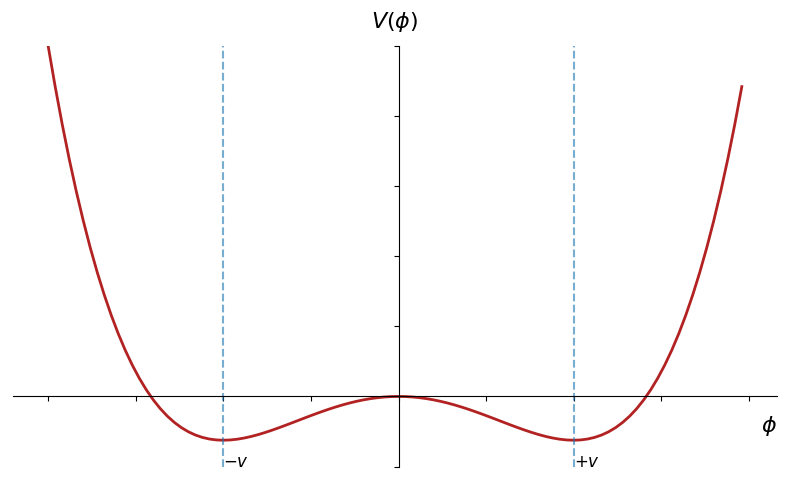
\includegraphics[width=\textwidth]{chapters/chapter1_theory/images/higgs-2d-vev.png}
    \caption{The one-dimensional Higgs potential where $\mu^2 <0$. The minima of this curve, known as the Higgs \gls{vev}, is indicated.}
    \label{fig:higgs-potential}
\end{figure}


\begin{equation} \label{higgs-lagrangian}
    \begin{aligned}
        \mathcal{L} &= \frac{1}{2}(\partial_{\mu}\phi)(\partial^{\mu}\phi) - V(\phi)\\
        &= \frac{1}{2}(\partial_{\mu}\phi)(\partial^{\mu}\phi) - \frac{1}{2}\mu^2\phi^2 - \frac{1}{2}\lambda\phi^4
    \end{aligned}
\end{equation}



%%%%%% Di-Higgs %%%%%%%%                
\section{Di-Higgs Production}


The analysis presented in this thesis searches for di-Higgs production - processes that pair produce Higgs bosons.   This process is rare, the total cross-section being {\color{red} 30} fb at 13 TeV center-of-mass energy.

\subsection{Production in the Standard Model}
In the standard model, several production modes pair produce Higgs bosons. \gls{ggF} is the most dominant with a cross-section of {\color{red} 33} fb, accounting for {\color{red} 89\%} of di-Higgs production. The next most dominant is Vector Boson Fusion. The remaining production modes, VHH, ttHH, and bbHH collectively comprise less than 5\% of di-Higgs production, and have a cross-section too small to make a meaningful contribution to the proposed analysis.

\subsubsection{Gluon-Gluon Fusion}

The predominant di-Higgs production mode is \gls{ggF}, in which the production is mediated by a quark loop. In the \gls{SM}, this proceeds through two diagrams at tree level, where the quark loop either forms a box or a triangle. The former directly pair produces two Higgs bosons while the latter pair produces via a virtual Higgs boson, making it sensitive to the Higgs self-coupling, $\lambda_{HHH}$.

\subsubsection{Vector Boson Fusion}
The second-most dominant HH production mode is \gls{VBF} ($qq \rightarrow HHqq$), in which two quarks scatter via the exchange of a virtual vector boson, $W$ or $Z$ (generally denoted $V$), and from that boson, a di-Higgs system is produced. This proceeds via three Feynman diagrams at tree level, shown in Figure \ref{fig:vbf_feyn}.

\begin{figure}[!thp]
    \begin{minipage}[c]{.31\textwidth}
        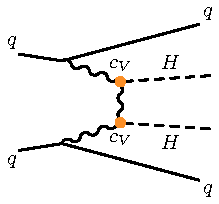
\includegraphics[width=\textwidth]{chapters/chapter1_theory/images/vbf_cv.pdf}
    \end{minipage}
    \begin{minipage}[c]{.31\textwidth}
        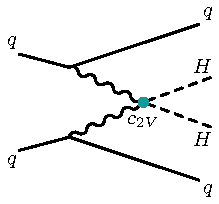
\includegraphics[width=\textwidth]{chapters/chapter1_theory/images/vbf_c2v.pdf}
    \end{minipage}
    \begin{minipage}[c]{.31\textwidth}
        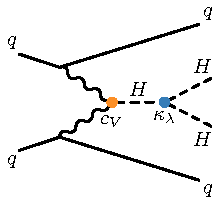
\includegraphics[width=\textwidth]{chapters/chapter1_theory/images/vbf_klambda.pdf}
    \end{minipage}

    \caption{Tree level Feynman diagrams for nonresonant VBF HH production \cite{vbf_4b}.}
    \label{fig:vbf_feyn}
\end{figure}

% TODO: Maybe this goes in analysis?
Despite the low cross-section of \gls{VBF} production, the unique kinematics make the channel appealing for searches. The diphoton \gls{VBF} channel was one included in the 2012 Higgs discovery. Notably, the \gls{VBF} quarks yield a high $m_{jj}$ system and are largely separated in $\eta$. The kinematics of \gls{VBF} di-Higgs production are similar to that of mono-Higgs. The major difference is that mono-Higgs searches take advantage of the low central jet activity by applying a veto. In $HH \rightarrow \gamma \gamma b\bar{b}$, however, the $H \rightarrow b\bar{b}$ system causes central jet activity, making such a veto impossible.


\subsection{Production Beyond the Standard Model}

Due to the small cross-section of $HH$ production, the LHC does not have sensitivity to \gls{SM} production. An enhancement to the cross-section, however, may be noticeable with the current data set and would indicate the presence of physics beyond the standard model. There are a variety of scenarios in which this could occur, both through a resonance and through non-resonant enhancements.

\subsubsection{Non-Resonant BSM Production}

Non-resonant enhancements to the $HH$ cross-section could occur through two major routes: deviations in couplings from \gls{SM} value, or the presence of couplings not predicted by the \gls{SM}.



\noindent\textbf{VBF}\\


\subsubsection{Resonant BSM Production}

Several \gls{BSM} theories predict particles that would decay to a pair of Higgs bosons, which would result in a resonant enhancement to the $HH$ cross-section. Notably, two Higgs doublet models extend the Higgs sector with the presence of a heavy scalar doublet \cite{THDM}. Among these models are the minimal supersymmetric extension of the \gls{SM} \cite{mssm}, twin Higgs models, and composite Higgs models \cite{compositeHiggs}.

\noindent\textbf{\gls{ggF}}\\
\indent

\noindent\textbf{VBF}\\
\indent Similarly to the searches for resonant ggF Higgs boson pair production, VBF HH
production involving an intermediate resonance may be considered. This kind of search would be complementary to the ggF searches, as in this case the vector bosons are the ones coupling to the new resonance, which then decays to a pair of Higgs bosons. However, this production mode is not
particularly well studied (Reference \cite{res_vbf} presents an analysis in the context of a model with warped extra dimensions), since its very small cross section poses a question on the ability of the LHC to impose significant constraints through this type of search.



